\documentclass[twoside,openright,a4paper,11pt,french]{article}
\usepackage[utf8]{inputenc}
\usepackage[french]{babel}
\usepackage[T1]{fontenc}
\usepackage{emptypage}
\usepackage{amsmath}

% Utilisation d'url
\usepackage{url}
\urlstyle{sf}

% Utilisation d'images, stockées dans le répertoire ./pics/
\usepackage{graphicx}
\graphicspath{pics/}

% Définition des marges
\usepackage{geometry}
\geometry{
  left=25mm,
  right=25mm,
  top=25mm,
  bottom=25mm,
  foot=15mm
}
\usepackage{listings}
\usepackage{color}

\definecolor{dkgreen}{rgb}{0,0.6,0}
\definecolor{gray}{rgb}{0.8,0.8,0.8}

\begin{document}

\pagestyle{plain}
\setlength{\parindent}{0pt}
% La page de garde
\thispagestyle{empty}

\begin{center}
       \noindent
       
\includegraphics[height=2.5cm]{./pics/uds.eps}       
       
       \vfill\vfill

    {\large \textsc{Licence 3 de Sciences, mention Informatique}}

    \bigskip\bigskip

    {\large \textsc{Programmation Orientée Objet 2 }}

    \vfill\vfill

% Titre du document
    {\huge \sc
      \begin{center} 
        Rapport sur le projet: \\
        détection des bords et vectorisation
      \end{center}}

    \vfill\vfill

    {\large Présenté par}

\medskip

% Identité des auteurs
    {\large Victor \textsc{Constans}}\\
    {\large Luigi  \textsc{Coniglio}}\\
\bigskip

\end{center}



% La table des matières
\parskip=0pt
\tableofcontents


\vspace{5cm}

%Start content

\section{Fichiers rendus et usage}
\subsection{Contenu du rapport}
L'objectif de ce rapport est d'abord celui d'illustrer la structure du
programme. Pour accelerer/simplifier l'utilisation du travail rendu, la partie
initiale de ce rapport décrit le contenu des fichiers et leur usage.

\subsection{Contenu de l'archive}
Après avoir ouvert l'archive {\it constans\_coniglio\_luigi.tar.gz} vous
trouverez les fichiers et repertoires suivants:
\smallbreak
\begin{itemize}
\item Ce rapport
\item Les fichier {\bf javimy.java} est le point d'entre du programme
\item Le repertoire {\bf gui} contiens tous les fichiers to du programme relatifs
      a l'interface graphique
\item Le repertoire {\bf filters} contient un package incluant tous les filtres 
      implemente dans la candre de ce projet
\item Le repertoire {\bf vectorization} contients la partie du programme dedie a
      la vectorisation d'une image
\end{itemize}

\bigbreak

\subsection{Usage}
Compilez le programme par le biais de la commande 
\colorbox{gray}{\lstinline[basicstyle=\ttfamily\color{black}]| javac javimy.java |}
Une fois termine la création des fichiers {\it .class} vous etes pret
a utiliser ce magnifigue logiciel: 
\colorbox{gray}{\lstinline[basicstyle=\ttfamily\color{black}]| java javimy |},

\vspace{1cm}
A l'execution il vous serait presente une interface graphique que vous
permettra de facon assez intuitive d'acceder aux different functions
du programme:

\begin{center}
% TODO image GUI %
\end{center}

\newpage 
\section{Filtres}
\subsection{Sobel, Prewitt, Roberts, etc...}
Description du principe de fonctionnement avec quelque image/example

\subsection{Canny}

\subsection{Gauss}
Description du principe de fonctionnement avec quelque image/example

\subsection{Segmentation}
La segmentation a l'objectif de partitionner un image en sections
(ensembles de pixels) sur la base de leurs propriete (couleurs,
intensite, ...). Dans le menu des filtres vous trouverez un bouton qui
va vous permet de realiser cette type de operation sur les couleurs
d'une image. 

L'algoritme utilise pour segmenter l'image est inspire du
partitionnement en {\it K-moyennes} (ou {\it k-means clustering} en
anglais). Ce type de partitionnement consiste a selectioner K couleurs
et assigner chaque pixel de l'image a le plus proche de ces couleurs.

\begin{figure}[h]
\centering
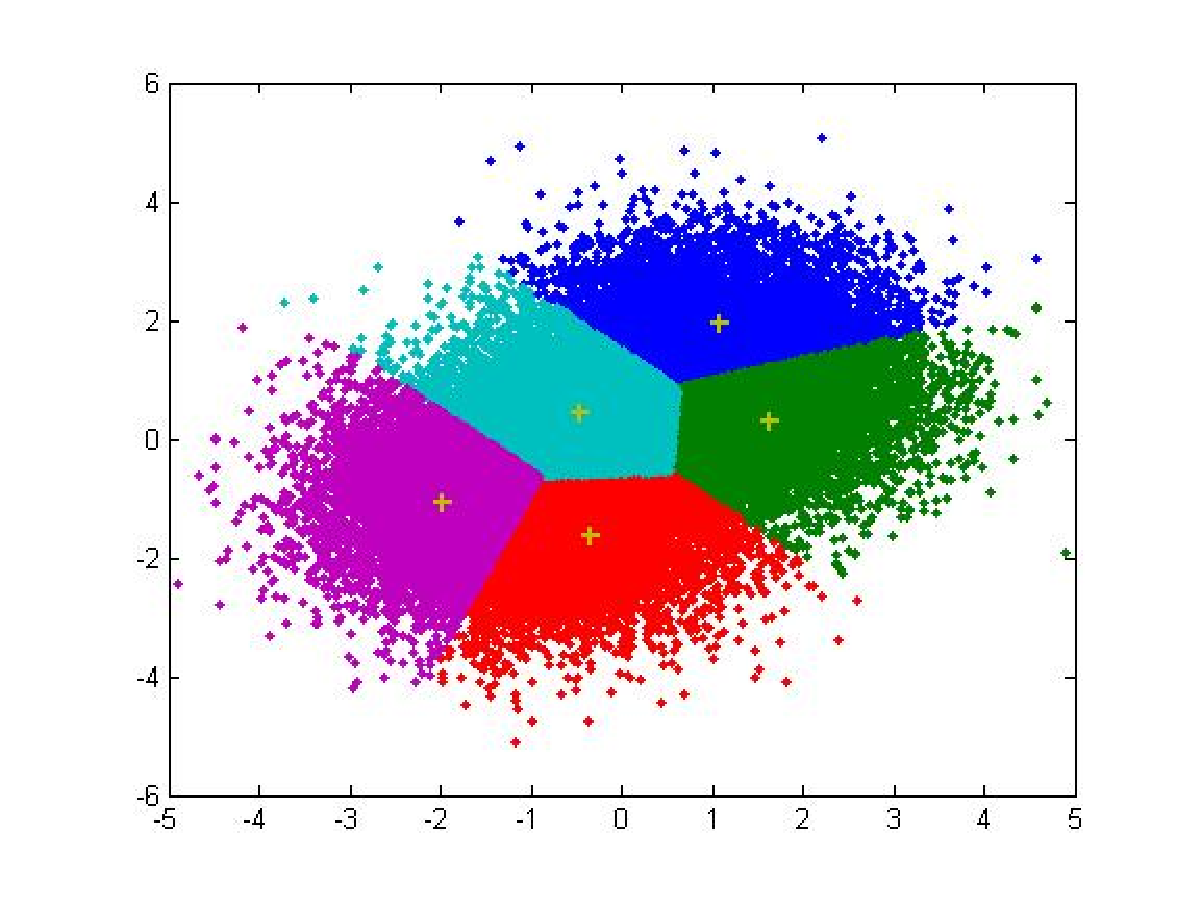
\includegraphics[width=8cm]{./pics/kmeans.eps}
\caption{Agrégation des pixels selon la plus courte distance avec les
K-moyennes (ici K = 5)}
\label{fig:routcidr}
\end{figure}

Les K couleurs sont apres modifie pour minimiser les distances avec
les pixel de l'image, les groupement par couleurs refait et ainsi de
suite jusq'a quand les K couleurs et le partitionnement des pixels
convergent. 

\subsection{Cluster-edges}
Cet filtre s'inscrit dans l'ensemble des filtres de detections des
bords. La particularite de ce filtre par rapport aux autres filtre de
detection des contours est que il n'effectue pas une simple detection
des bords mais, plus precisement, il determine les limites entre
differents zones de couleurs. 
Les limites entre deux zones de couleurs sont represente par des
chemin colore. A chaque bord correspond un chemin d'un couleur
different.



\newpage

\section{Vectorisation} 
La vectorisation permet d'exporter une image sous la forme d'un
fichier {\it .svg}. Pour 


\begin{itemize}
\item Un utilisateur ne peut pas visionner une vidéo qui n'a pas été diffusé,
par contre il peut le sélectionner (le mettre dans les favoris) par exemple
pour un visionnage futur. Trigger {\it ValidView}.

\item Un utilisateur ne peut pas visionner une vidéo qui a dépassé la date de
validité (même s'il n'a pas encore été archivée). Trigger {\it ValidView}.

\item Si la date de disponibilité n'est pas passée, une vidéo ne peut pas être supprimée. 
      Trigger {\it WaitExpiration }.

\item Comme spécifie le sujet: {\it "Après une diffusion, une vidéo sera
accessible sur le site en replay pendant au moins 7 jours"}. 
\footnote{NB: la deuxième contrainte demande dans le sujet ({\it"Si une diffusion d’une émission est
ajoutée, les dates de disponibilités seront mises à jour.  La nouvelle date de
fin de disponibilité sera la date de la dernière diffusion plus 4 jours."})
n'implique pas que cette contrainte soit satisfaite (p.ex. il ne couvre pas les
opérations d'UPDATE sur la table {\it Video}).} 
Trigger {\it BadExpiration}.

\item La date (année) de première diffusion d'une vidéo ne doit pas être
supérieure la date de la première diffusion dans la table {\it Diffusion}.
Triggers {\it FirstDiffusionCheck} et {\it VideoWasDiffused}.

\item  Au moment de sa création, le champ Time d'un visionnage ne peut pas être
supérieure à la date actuelle (SYSDATE): on interdit les visionnages "dans le
futur".
\footnote{C'est le cas typique d'une contrainte qui pourrait être remplacé par
l'intervention de l'application web (côté serveur) dans le choix de la date du
visionnage.}
Trigger {\it ValidView}.



\end{itemize}

%End content

\end{document}
